\documentclass[
    NAME={Dr. Helga Ingimundardóttir},
    EMAIL={helgaingim@hi.is},
    FACULTY={Iðnaðarverkfræði},
    TITLE={Hagnýt hæfni í brennidepli},
    SUBTITLE={Endurskoðun á námskeiði í Viðskiptagreind},
    SEMINAR={Ráðstefna kennsluakademíunnar},
    DATE={22 nóvember, 2024},
    WIDE={true},
    ICELANDIC={true}
]{HI-LaTeX/hi-beamer}
\usepackage{multimedia}
\usepackage{tikz}
\usetikzlibrary{positioning, arrows, shapes, fit}
\usepackage{textcomp}

\newcommand{\customframe}[3][]{
    \usebackgroundtemplate{
        \tikz[overlay,remember picture]
        \node[opacity=0.3, at=(current page.center)] {
            \includegraphics[width=\paperwidth,height=\paperheight]{#2}
        };
    }
    \ifx&#1&
        \section{#3}
    \fi
    \addtobeamertemplate{frametitle}{}{} % Adjust the frametitle position for this slide only
    \begin{frame}[plain]{#3}
        #1
    \end{frame}
    \addtobeamertemplate{frametitle}{}{} % Reset the frametitle template to default
    \usebackgroundtemplate{}  % Reset the background for the following frames
}

\begin{document}

% Section: Inngangur
\section{Inngangur}
\begin{frame}{Inngangur}
    \begin{block}{Hvað er Viðskiptagreind?}
        Viðskiptagreind (VG) nýtir gögn og tækni til að veita innsýn sem styður upplýstar \alert{gagnadrifnar} ákvarðanir, eykur skilvirkni og bætir rekstur.
    \end{block}
    \vspace{0.5cm}
    \begin{block}{Valnámskeið (M-áfangi) í iðnaðarverkfræðideild}
        Sérstaklega hannað fyrir 3ja árs iðnaðarverkfræðinema með áherslu á:
        \begin{itemize}
            \item Að hámarka flókin kerfi með gagnaöflun.
            \item Að samþætta greiningu við stefnumótandi ákvarðanir.
            \item Að þróa hæfni til nýsköpunar og samkeppnisforskots.
        \end{itemize}
    \end{block}
\end{frame}


\begin{frame}{Hvað var vandamálið?}
    \begin{itemize}
        \item Misræmi milli hæfni nemenda og atvinnulífs
        \item Endurgjöf frá útskrifuðum nemendum:
        \begin{itemize}
            \item Áhersla á \textit{Learning-by-Doing} (LbD)
            \item Betri notkun á \textit{GitHub} fyrir verkstjórn og samvinnu
        \end{itemize}
        \item Innsýn úr vinnustofu LOUIS verkefnisins:
        \begin{itemize}
            \item Endurskoðun byggð á \textit{Understanding by Design} (UbD)
        \end{itemize}
    \end{itemize}
\end{frame}

% Section: Aðferð
\section{Aðferð}
\begin{frame}{Hver var lausnin?}
    \begin{itemize}
        \item Verkefnamiðuð námsaðferð (\textit{Problem-Based Learning}, PBL)
        \item Þróun \textit{Capstone}-verkefna:
        \begin{itemize}
            \item Samþætting hagnýtrar notkunar við raunverulegar áskoranir
            \item Áhersla á gagnvirka og rökstudda hugsun
        \end{itemize}
        \item Uppbygging námskeiðs:
        \begin{itemize}
            \item Lotur: gagnasiðfræði, mállíkön, klösun og ferlagreining
            \item Lokaverkefni sem samþættir öll viðfangsefni
        \end{itemize}
    \end{itemize}
\end{frame}

\begin{frame}
    \frametitle{Uppbygging námskeiðs}
    Námskeiðið er byggt á \alert{nýjustu straumum} í faginu og samanstendur af sex\footnote{Árið áður náði námskeiðið aðeins yfir fyrstu 5 atriðin sem voru teygð yfir alla önnina.} lotum:
    \begin{enumerate}
        \item Gagnasiðfræði
        \item Leiðbeint nám og reiknifræði
        \item Mállíkön
        \item Klösun (unsupervised learning)
        \item Ferlagreining (process mining)
        \item Samantektarverkefni (Capstone)
    \end{enumerate}
    \begin{itemize}
        \item Í gegnum allt námskeiðið var unnið með gögn frá sama fyrirtæki. 
        \item Í hverri lotu var lögð áhersla á afmarkaða aðferðafræði sem beitt var á gögnin.
    \end{itemize}
\end{frame}

\begin{frame}{Samantektarverkefni}
    \begin{columns}
        \begin{column}{0.7\textwidth}
            Capstone verkefnið sameinar lotur námskeiðsins í eina heildstæða reynslu.
            Nemendur unnu í samstarfi við \alert{Tixly Ticketing} og notaðu raunveruleg gögn til að útbúa tæknilega skýrslu og kynningu.
            \newline\newline
            Þetta verkefni hermir eftir starfsháttum faglegs VG ráðgjafa þar sem áherslan er á hagnýta notkun greiningarhæfni í raunverulegu viðskiptasamhengi.
        \end{column}
        \begin{column}{0.3\textwidth}
            
\includegraphics[width=\linewidth]{figures/company}
        \end{column}
    \end{columns}
\end{frame}

\begin{frame}{Skipulag námskeiðsins}
    \begin{table}
        \begin{tabular}{ccc}
            \textbf{Vika} & \textbf{Námsefni} &  \\
            1-3 & Gagnasiðfræði & 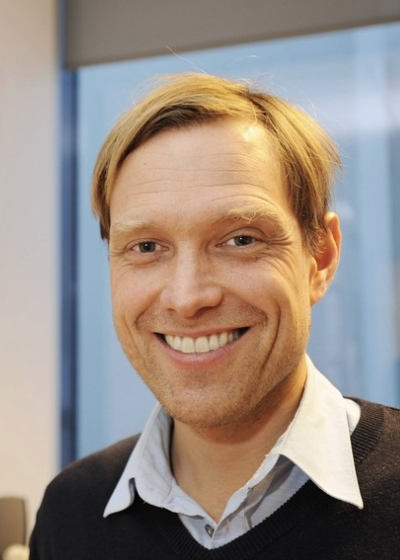
\includegraphics[height=.08\textheight]{figures/hah}\\
            4-5 & Leiðbeint nám og reiknifræði & 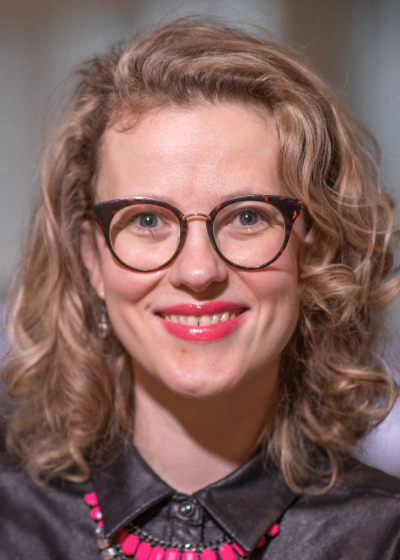
\includegraphics[height=.08\textheight]{figures/helgaingim} \\
            6-7 & Mállíkön                                   & 
\includegraphics[height=.08\textheight]{figures/hafsteinne} \\
            8-9 & Klösun (unsupervised learning) & 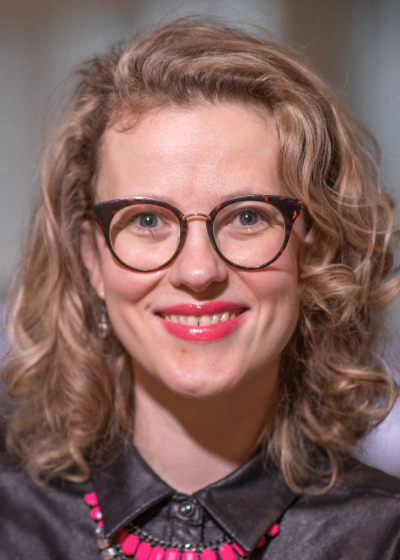
\includegraphics[height=.08\textheight]{figures/helgaingim} \\
            10-11 & Ferlagreining (process mining)            & 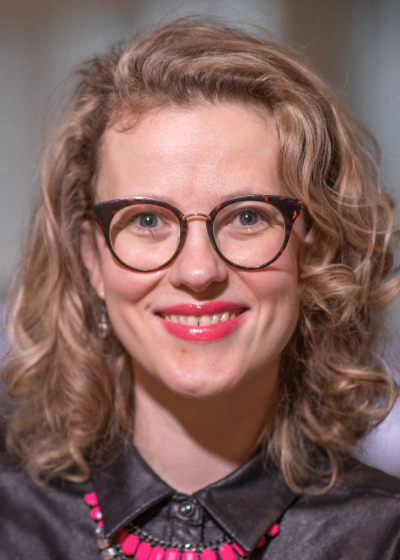
\includegraphics[height=.08\textheight]{figures/helgaingim} \\
            12-15 & Capstone verkefni (með páskafrí) & 
\includegraphics[height=.08\textheight]{figures/company}    
        \end{tabular}
    \end{table}
\end{frame}

\begin{frame}{Framvinda námskeiðsins}
    \begin{figure}
        \centering
        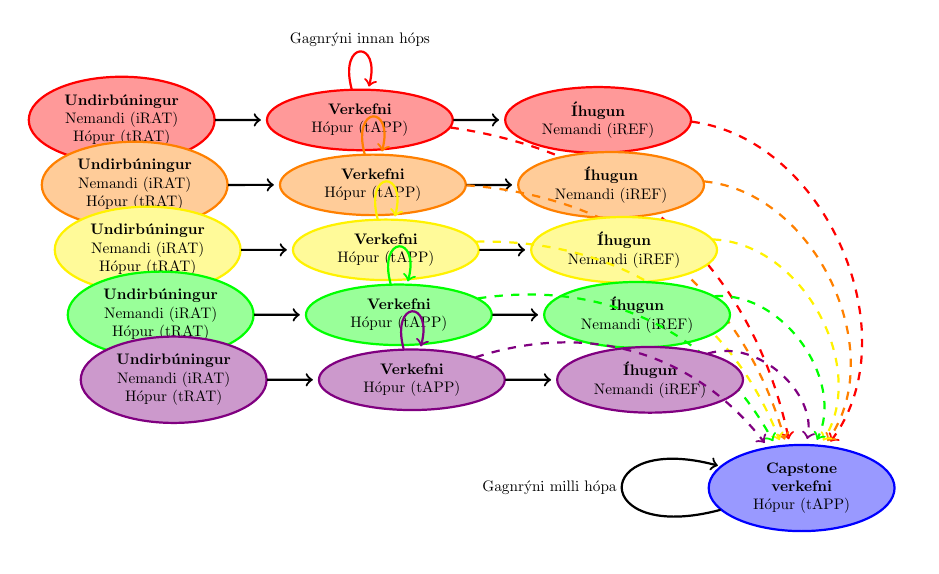
\begin{tikzpicture}
            [scale=0.55, transform shape,
            node distance=5.5cm,
            auto,
            block/.style={
                ellipse,
                draw,
                thick,
                fill=green!40,
                text width=2.8cm,
                align=center,
                minimum height=1cm,
                minimum width=3.0cm
            },
            line/.style={
                draw, thick, ->, shorten >=2pt
            },
            dashedline/.style={
                draw, thick, ->, dashed, shorten >=2pt
            },
            red/.style={block, draw=red, fill=red!40},
            orange/.style={block, draw=orange, fill=orange!40},
            yellow/.style={block, draw=yellow, fill=yellow!40},
            green/.style={block, draw=green, fill=green!40},
            violet/.style={block, draw=violet, fill=violet!40},
            blue/.style={block, draw=blue, fill=blue!40}
            ]

            % Capstone node
            \node[blue] (capstone) at (16cm,-10cm) {\textbf{Capstone verkefni}\\Hópur (tAPP)};
            \draw [line] (capstone) edge[loop left] node {Gagnrýni milli hópa} (capstone);

            \foreach \color/\pos in {red/1, orange/2, yellow/3, green/4, violet/5}{
                \node[\color] (RAT\pos) at (\pos*.3cm,-\pos*1.5cm) {\textbf{Undirbúningur}\\Nemandi~(iRAT)\\Hópur (tRAT)};
                \node[\color, right of=RAT\pos] (APP\pos) {\textbf{Verkefni}\\Hópur (tAPP)};
                \node[\color, right of=APP\pos] (REF\pos) {\textbf{Íhugun}\\Nemandi~(iREF)};

                \path [line] (RAT\pos) -- (APP\pos);
                \path [line] (APP\pos) -- (REF\pos);

                % Loop only for the first node with text
                \ifnum\pos=1
                    \draw [line,draw=\color] (APP\pos) edge[loop above] node {Gagnrýni innan hóps} (APP\pos);
                \else
                    \draw [line,draw=\color] (APP\pos) edge[loop above] (APP\pos);
                \fi

                \path [dashedline,draw=\color] (APP\pos) to[bend left=35] (capstone);
                \path [dashedline,draw=\color] (REF\pos) to[bend left=60] (capstone);
            }
\end{tikzpicture}

    \end{figure}
\end{frame}

\begin{frame}{Námsmat}
    \begin{columns}[T] % align columns
        \begin{column}{.48\textwidth}
            \begin{block}{Lotur (50\% af heildareinkunn)}
                \begin{itemize}
                    \item Hver lota: 10\%
                    \begin{itemize}
                        \item iRAT: 1\%
                        \item tRAT: 1\%
                        \item tAPP: 4\%
                        \item iREF: 4\%
                    \end{itemize}
                \end{itemize}
            \end{block}
        \end{column}%
        \hfill%
        \begin{column}{.48\textwidth}
            \begin{block}{Capstone (50\% af heildareinkunn)}
                \begin{itemize}
                    \item Gagnrýni: 20\%
                    \begin{itemize}
                        \item Endurgjöf nemenda: 10\%
                        \item Kennaraúttekt: 10\%
                    \end{itemize}
                    \item Kynning: 20\%
                    \item Tæknileg skýrsla: 30\%
                    \item Einstaklingsskýrsla: 10\%
                    \item Einkunn frá fyrirtæki: 20\%
                \end{itemize}
            \end{block}
        \end{column}%
    \end{columns}
\end{frame}

\begin{frame}{Hvernig loturnar nýtast fyrir Capstone verkefnið}
    \begin{block}{Undirbúningsverkefni}
        \begin{itemize}
            \item Nemendur „brainstorma“ um hvernig aðferðafræðin gæti nýst í hópverkefninu.
        \end{itemize}
    \end{block}
    \begin{block}{Mat á hópverkefnum í hverri lotu}
        \begin{itemize}
            \item Verkefni metin eftir matskvarða: byrjandi/í þróun/árangur/framúrskarandi.
            \item Sami kvarði notaður fyrir Capstone, svo nemendur sáu hvar bæta mætti fyrir lokaútfærslu.
        \end{itemize}
    \end{block}
    \begin{block}{Sjálfsígrundunarverkefni í lokinn}
        \begin{itemize}
            \item Nemendur skráðu hvað þyrfti að bæta/breyta, án þess að leysa það strax.
        \end{itemize}
    \end{block}
\end{frame}



% Section: Niðurstöður
\section{Niðurstöður}
\begin{frame}{Niðurstöður}
    \begin{itemize}
        \item Betri þátttaka nemenda:
        \begin{itemize}
            \item Nær fullkomin mæting, jafnvel án mætingarskyldu
        \end{itemize}
        \item Endurgjöf nemenda:
        \begin{itemize}
            \item Nám krefjandi en lærdómsríkt
            \item Betri skilningur á raunverulegum verkefnum
        \end{itemize}
        \item Samantektarverkefni:
        \begin{itemize}
            \item Verkefni tengd atvinnulífi sem stuðla að hagnýtri reynslu
        \end{itemize}
    \end{itemize}
\end{frame}

% Section: Umræður
\section{Umræður}
\begin{frame}{Umræður og næstu skref}
    \begin{itemize}
        \item Áhersla á hópmyndun og traust:
        \begin{itemize}
            \item Þróun nýrrar lotu í upphafi námskeiðs
        \end{itemize}
        \item Heildarsýn á verkefnið:
        \begin{itemize}
            \item Lögð áhersla á að teymi hugsi heildrænt frá upphafi og það sé einn rauður þráður í gegnum allar lotur.
            \item Þetta auðveldar þeim að púsla saman niðurstöðum í Capstone verkefninu og kynna þær fyrirtækinu.
        \end{itemize}        \item Áhrif á atvinnulífið:
        \begin{itemize}
            \item Fyrirtæki nýta niðurstöður nemenda
        \end{itemize}
    \end{itemize}
\end{frame}

% Thank You Slide
\customframe[
\vspace{0.6\textheight}

\hfill Takk fyrir! Spurningar?]{figures/github-classroom.jpg}{$\quad$}


\end{document}
